\chapter{General introduction}
\newpage

Life began about four billion years ago with the encapsulation of self-replicating RNA in a lipidic membrane \cite<e.g.>{orgel1968}. Simple as these probionts were, they did not have any means of locomotion and thus relied in full on the currents to deliver the nutrients required to replicate. As organisms evolved, they began to assert an increasing amount of control over their environment. A primitive example can be found in chemotaxis, where ciliae and flagellae, coupled with simple biochemical sensors allow the organism to follow biochemical gradients and thus actively gather nutrients.

Because flagellar motion is limited to either tumbles - random reorientation movements - or runs, the pathway linking these flagella to the biochemical sensors consists of only a few steps. With the advent of more advanced sensory and motoric systems, both the amount of information available to drive behaviour as well as the amount of possible behaviours available increased tremendously. As direct biochemical links between perception and action were no longer sufficient, simple neural network evolved to process the sensory signals allowing for abstract decisions about movement. Because organisms became more complex, these networks evolved into a complete (central) nervous system, culminating in the cerebral cortex.

In most higher organisms, including humans, the amount of data collected by the sensory organs is enormous, the visual system alone generating between $10^7$ and $10^9$ bits per second \cite{koch2006,kelly1962}. The nervous system, and the cerebral cortex in particular, seem to use probabilistic models to compress the vast amount of the incoming sensory data \cite{zhaoping2006}. The principal idea behind these models being that they reduce redundancy in the input by knowledge about the statistics of the natural world.

Predictive models, or maps, on the spatial organization of the environment are of particular interest to an organism, since they provide for example probable locations of food and predators. To use these maps, the brain needs to know both the location and orientation of the body within the environment. In this thesis, we will investigate how the brain processes the available sensory signals in the perception of gravity as well as in the internal estimation of self-motion. The goal is to build computational models and perform thorough psychometric testing in order to examine the constraints that physics and biology impose on the interaction between the vestibular and other sensory systems. 

In the following section, sensory sources for gravity and self-motion perception are described in more detail. We then elaborate on how these signals may be used and integrated in the brain, and conclude the chapter with methods for studying the processing of these signals. 
 


\section{Sensory signals for navigation}

The signals used for self-motion and orientation perception, can be split in two broad categories: absolute signals and relative signals. Absolute signals, such as landmarks, can be used to directly estimate the location and orientation of an animal while relative signals, such as acceleration, first need to be (mathematically) integrated (i.e. dead reckoning or path integration) and then used to update previous estimates of position and orientation. In the following sections the sensory system involved in position and orientation estimation will be introduced.

\subsection{Vestibular system}

While many sensory organs supply information that can be used to estimate position and orientation, there is one sensory system that evolved specifically for this purpose: the vestibular system (\figref{intro:vestibular}). It contains two sensory components, the semicircular canals and the otoliths. These sensory organs are sensitive to angular velocity and linear acceleration, respectively. Both are located in the labyrinth of the temporal bone in the inner ear.

\begin{figure}
    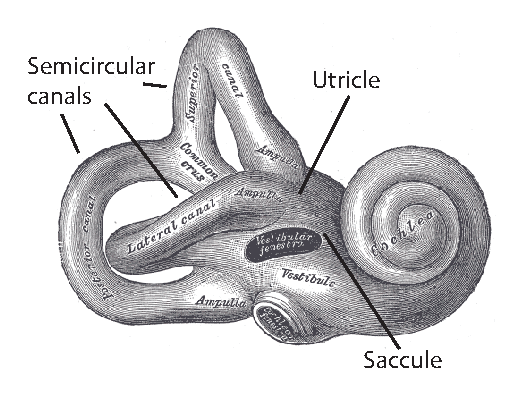
\includegraphics[width=0.5\textwidth]{src/intro/figures/vestibular.pdf}
    \caption{Schematic view of the inner ear complex consisting of the auditory system (cochlea) and the vestibular system. The vestibular system has three angular velocity (semicircular canals) and two linear acceleration (saccule and utricle) sensors. Image adapted from \protect\citeNP{gray1918}.}
    \label{intro:vestibular}
\end{figure}


\subsubsection{Semicircular canals}

The semicircular canals measure the three-dimensional rotational velocity of the head. Each side of the head contains three orthogonally oriented canals allowing for rotation to be perceived in all three dimensions. Each of the six canals consists of a circular tube filled with a fluid known as endolymph (see \panelref{intro:fig:canals}{A}). One part of the tube, the ampulla, is a bit thicker than the rest and contains a membrane, the cupula, which separates the fluid. When the head rotates, the fluid stays behind because of its inertia which in turn causes the membrane to deflect (see \panelref{intro:fig:canals}{B}). While the inertial fluid motion suggests that the cupula should be sensitive to angular acceleration, reactive forces resulting from the fluid motion, such as endolymph viscosity and cupular elasticity,  cause the cupular deflection to reflect angular velocity instead \cite{goldberg2012}.

\begin{figure}
    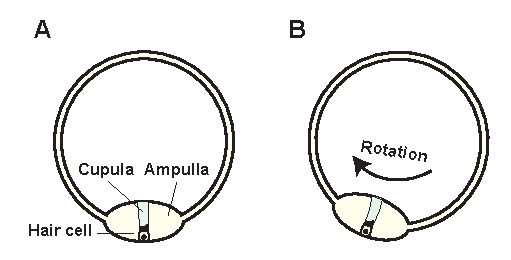
\includegraphics[width=1.0\textwidth]{src/intro/figures/canals.pdf}
    \caption{Detailed view of a semicircular canal \panel{A} in rest and \panel{B} during rotation. Inertia of the endolymph in the canal causes the cupula to deflect during rotation.}
    \label{intro:fig:canals}
\end{figure}

The deflection of the cupula is transduced by special hair cells which are partially embedded in the cupula. These hair cells contain bundles of small protrusions, or hairs, on their apical surface. Each bundle contains several smaller stereocilia mechanically linked to one larger kinocilium \cite{pickles1984}. When the stereocilia are stretched towards the kinocilium the links cause cation channels (mechanoelectric transducers or METs) to open and the membrane to depolarise. Glutamate is then released into the synapse and causes the afferent neuron to depolarise and, after sufficient depolarisations, to generate action potentials \cite{purves2012}. These action potentials transmit the angular velocity sensed by the canals to the central nervous system through the vestibulocochlear nerve.

Initially, the afferent signal closely follows rotational velocity, as opposed to acceleration. During sustained rotation, the elasticity of the cupula returns it to its resting position with causes the rotational signal to subside slowly. This is partly compensated for through velocity storage in the central nervous system \cite{goldberg2012}. The canals are only sensitive to changes in orientation, as their circular nature makes them insensitive to the effects of linear acceleration and gravity \cite{goldberg2012}. 


\subsubsection{Otoliths}
The linear acceleration and gravitational forces are measured by the two otolith organs on either side of the head: the saccule and the utricule. Each otolith consists of an endolymph filled compartment containing calcium carbonate crystals known as otoconia (\panelref{intro:fig:otoliths}{A}). Due to their high inertia, these otoconia fall behind during linear acceleration (\panelref{intro:fig:otoliths}{B}), and move ahead during deceleration. In addition, they fall downward as a result of the gravitational field (\panelref{intro:fig:otoliths}{C}). The otoconia are mounted on top of a flexible polysaccharide gel, in which hair cells, similar to those found in the semicircular canals, are partly embedded \cite{goldberg2012}.  

Einstein's equivalence principle states that  it is not possible to measure forces caused by linear acceleration and by gravity independently. The signal coming from the otoliths is therefore proportional to the combination of these forces \cite{fernandez1976b}, which is commonly referred to as the gravito-inertial force (GIF). Compared to the three semicircular canals, which are able to sense rotation in three dimensions due to their orthogonal organization, either side of the head only contains two otolith organs. It is still possible to sense the gravito-inertial force in three dimensions because the otolith organs are curved, and the orientation of the hair cells determined the direction of sensitivity \cite{goldberg2012}.

\begin{figure}
    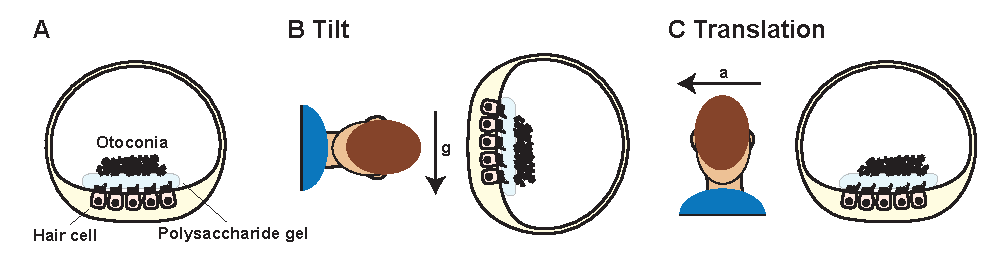
\includegraphics[width=1.0\textwidth]{src/intro/figures/otoliths.pdf}
    \caption{Detailed view of an otolith \panel{A} in rest, \panel{B} during head tilt, and \panel{C} during linear acceleration. The high inertia of the otoconia keeps them from moving rapidly during both head tilt as well as linear acceleration. As the effect is physically identical in either case, head tilt and linear acceleration cannot be disambiguated based on the otolith signal alone.}
    \label{intro:fig:otoliths}
\end{figure}

For many actions, the brain needs to disentangle the contributions of gravity and linear acceleration to the gravito-intertial force. For example, the linear vestibulo-ocular reflex (LVOR) that stabilizes gaze during translation should be sensitive to translation while ignoring gravity. Under normal circumstances, the brain is able to perform this task well \cite{merfeld1995}, but during extreme conditions such as in airplanes or space flight errors might occur. The somatogravic illusion \cite{glasauer1995} is an example of a disambiguation error. In this illusion an airplane accelerates forward which causes an inertial force in the opposite direction. The direction of the resulting GIF will therefore be in between gravity (downward) and the intertial force (backward). The brain erroneously interprets the (majority of the) GIF as being caused by gravity, leading to the perception of "nose-up" pitch tilt.

Various theories have been proposed as to how the brain might solve the tilt-translation ambiguity. The frequency segregation hypothesis, for example, makes use of the fact that when stationary, the only force we experience is gravity. In this case, sustained (low frequency) accelerations should be  attributed to gravity, while the high frequency components should be attributed to translation \cite{paige1991, telford1997}. Other models keep track of the expected direction of gravity by integrating over the vector product of gravity and angular velocity from the semi-circular canals, and subtracting that signal from the otolith signal to obtain an estimate of linear acceleration. Because the semi-circular canals play a crucial role in these models, they are known as multisensory integration models \cite{mayne1974,ormsby1977}. Merfeld and Zupan \citeyear{merfeld1995,merfeld2002} further refined the multisensory integration model by explicitly stating that the brain uses an (internal) model of the physical world to resolve the tilt-translation ambiguity.

The disambiguation of linear acceleration and gravity is not solely based on vestibular inputs, but also takes the range of possible movements into account. For example when moved on a linear sled, the probability of a participant perceiving tilt is greatly reduced \cite{wertheim2001}, indicating that cognitive processes also influence disambiguation.


\subsection{Somatosensory}
The gravito-inertial force (GIF) caused by a combination of gravity and linear acceleration is not only detected by the vestibular system, but also sensed by other sensory systems. Early evidence that non-vestibular sources were used by the brain came from DeKleyn and Versteegh \citeyear{dekleyn1933} who showed that inertial reflexes still occurred after removal of the otolith organs.

Since then, the contribution of specific organs to GIF perception has been demonstrated. In 1992, \citeauthor{mittelstaedt1992} rotated supine participants along their naso-occipital axis, causing the centrifugal force to act on somatic GIF sensors  but not on the otoliths. In nephrectomised participants, the perceived direction of gravity relied less on the centrifugal force compared to controls, suggesting that the kidneys play a crucial role in perception of the gravito-intertial force. Further evidence came from Trousselard \citeyear{trousselard2004}, who showed that the perception of gravity in a tilted position depends on whether the stomach is full or empty. In addition, reducing somatosensory cues, by applying a body cast, also affects the perception of gravity \cite{trousselard2004}.  Similar results have been obtained for many other visceral factors, such as the blood vessels \cite{vaitl2002}, and spinal axis fluid \cite{vaitl1997}.


\subsection{Visual}
Even though the vestibular and somatosensory systems directly measure the gravito-inertial force, orientation and navigational information can also be extracted from the visual system. In many cases, especially when the low latency of the vestibular signal is not required, the visual signal even overshadows the vestibular one \cite{wright2005,gaerlan2012}.

\subsubsection{Vection}
When we move through the environment, the image of the world on our retina shifts. This large-field shift pattern, also known as optic flow, depends on the movement being made. Lateral translation (\panelref{intro:fig:vection}{A}) for example causes a different pattern than roll rotation (\panelref{intro:fig:vection}{B}). At the turn of the 19th century von Helmholtz \citeyear{vonhelmholtz1867} recognized the importance of these flow signals for self-motion perception. In some cases the optic flow signal is so strong that it causes a percept of self-motion in stationary participants, called vection \cite{dichgans1978}. This is experienced, for example, when sitting on the train and a neighbouring train starts to move. This effect is much less likely to occur when e.g. on the platform, suggesting that the vection signal is integrated with prior knowledge about the environment before causing self-motion perception \cite{andersen1985,lepecq1995}


\begin{figure}
    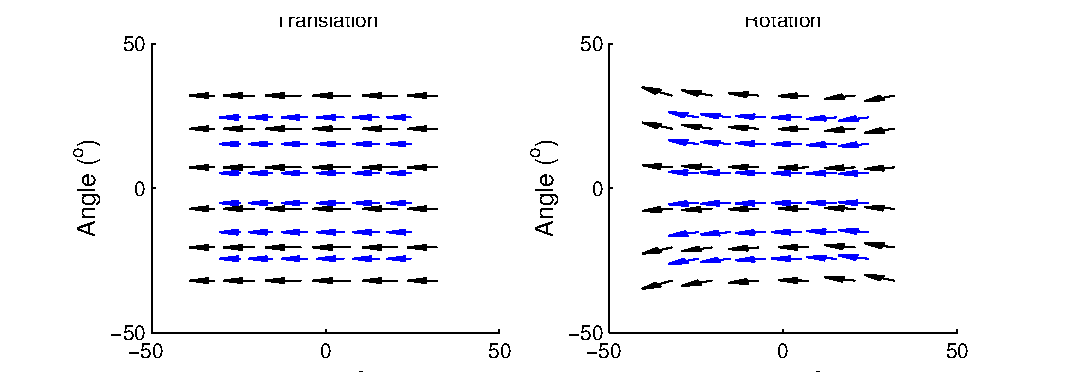
\includegraphics[width=1.0\textwidth]{src/intro/figures/optic_flow.eps}

    \caption{Vection pattern during \panel{A} lateral translation and \panel{B} rotation. During translation nearby targets (red) have a larger retinal displacement compared to far away ones (blue). Retinal displacement across rotation does not depend on target distance. }
    \label{intro:fig:vection}
\end{figure}

Similar retinal shifts are also observed during movement of the eyes or head. When interpreting optic flow the brain needs to distinguish object- from self-motion, this process is called optic flow parsing. One strategy is to use extra-retinal cues such as the vestibular, and somatosensory signals to subtract out the retinal stimulation due to self-motion \cite{wertheim1994,wexler2001,macneilage2012}.

While the extra-retinal information does contribute to optic flow parsing, the existence of vection \cite{dichgans1978} suggests that the brain can parse optic flow using a purely visual approach \cite{rushton2005,warren2007}. Warren and Rushton \citeyear{warren2009} have shown that the brain indeed uses the global pattern of retinal motion caused by self-motion to parse optic flow. Even though global retinal flow patterns are used to disambiguate between object- and self-motion, it does not mean that a percept of self-motion, i.e. vection, exists. Research has shown that vection can take up to 30s to establish, but that purely visual optic flow parsing occurs within 1s \cite{warren2009}.

\subsubsection{Landmarks}
In addition to relative cues, the brain seems to use absolute cues in both the perception of gravity and self-motion. For the perception of gravity, it makes use of the fact that many lines within the world are aligned with either the horizon or gravity (\panelref{intro:fig:treeframe}{A}). Straight lines therefore acts as a priors attracting the perceived direction of gravity towards them. A special case is the rod-and-frame illusion (\panelref{intro:fig:treeframe}{B}), where the perceived angle of a rod relative to gravity is affected by the orientation of the frame that contains it \cite{witkin1948}. 

\begin{figure}
	\includegraphics[width=1.0\textwidth]{src/intro/figures/treeframe.pdf}
	\caption{\panel{A} Trees are aligned with gravity, making them ideal cues for orientation. \panel{B} The rod-and-frame illusion; even though the frame is rotated, participants might perceive the line as being slanted.}
	\label{intro:fig:treeframe}
\end{figure}

Similarly, our position within the world can be established using world-fixed landmarks. With the exception of animals and vehicles, most items in the world rarely change position. By comparing our current visual scene (e.g. Sequoia trees in \panelref{intro:fig:treeframe}{A}) with our knowledge about the environment we can determine our location (in this case northern California). Because the experiments outlined in this thesis were performed in near darkness, these absolute navigational cues can be considered less relevant. 


\subsubsection{Oculomotor}
Self-motion is typically accompanied by eye movements that help to improve dynamic visual acuity and reduce retinal slip. In \Chapter{p3} of this thesis, we explore whether these eye movements may have a reversed role, providing cues about self-motion perception beyond optic flow parsing. 

In \citeyearNP{guedry1963}, \citeauthor{guedry1963} reported a substantial underestimation of displacement when their observers watched a small body-fixed target compared to displacements in the dark. Because of the VOR, eye movement in darkness are larger than those in the body-fixed condition. The underestimation in the body-fixed condition can therefore be interpreted as the involvement of eye movements, although the authors did not suggest this 
Studies on postural sway also indicate a role of eye movement is self-motion perception. Making eye movements causes postural sway to increase, suggesting that eye movements influence self-motion perception \cite{glasauer2005,rodrigues2015}.

One complication is that the magnitude, $e$, of these eye movements not only depend on the translation amplitude, $T$, but also on the fixation depth, $d$. Oculomotor cues to depth include binocular vergence angle and accommodation, both most robust for less fixations than a meter or so away. When fixating position $(x, d)$, the eye position at starting position is $e_0 = \arctan(d/x) \approx d/x$. By subtracting the eye position after the translation, $e_1 = \arctan(d/(x+T)) \approx d/(x+T)$, we obtain the eye movement amplitude, $e \approx d/T$. In \Chapter{p4} we explore whether the brain takes this geometry into account and compensates for fixation depth when using eye movements in self-motion perception. Fixation depth plays also a crucial role in \Chapter{p2}, in which the the effects of eye and head movements on spatial updating are investigated.


\section{Reflexive uses for the self-motion}
While vection is a valuable cue to self-motion perception, the brain wants to minimize vection because it blurs the image on the fovea, which hampers visual perception. Several reflexive mechanisms attempt to keep stable fixation to avoid image blurring during self-motion. Two such mechanisms are the vestibulo-ocular reflex, the VOR \cite{goldberg2012}, and the optokinetic reflex, the OKR \cite{purves2012}.

The vestibulo-ocular reflex (VOR) is driven by the short-latency vestibular signal and compensates for both rotation and translation of the head. The rotational and translational part of the VOR have their own dedicated reflex arcs. The translational VOR, or TVOR, is driven by the otolith signal while the rotational VOR, or RVOR, is mainly driven by the semicircular canals. The RVOR operates during head rotation by counter rotating the eyes in the opposite direction to the head. Because its gain is about one, eye velocity is about equal, but of opposite sign, to the head velocity \cite{goldberg2012}. The TVOR operates during head translation, when the head moves orthogonally to the line of sight. In contrast to the RVOR, the TVOR needs to take fixation depth into account. Simple geometry shows that the ideal TVOR response is inversely proportional to fixation distance, $e_{vor} = \arctan(d/T)$. As a result, no compensatory eye movements are required when fixating targets at infinity to maintain a stable retinal image. 

The optokinetic reflex is driven by optic-flow, and also compensates for both translational and rotational movement. Because the cells driving the OKR are more sensitive to slow motion, the OKR compensates predominantly for the low frequency components of movements. While the VOR dies away during sustained rotation, the OKR remains because it is sensitive to constant velocity stimuli \cite{soodak1988}.

The eye movements that are induced by the OKR and the VOR consist of two parts; a slow-phase pursuit-like movement which keep the eyes on target and quick-phase saccades which quickly move the eyes back after they lost track due to physical constraints of the oculomotor system \cite{goldberg2012}.

\section{Integration of signals for action and perception}

While reflexes by definition depend on minimally processed sensory signals, higher animal functions can rely on more elaborate processing. One such processing step is determining the underlying physical cause of a sensory signal. Multiple sensory systems provide information about the same physical quantity. For example, both the visual and the vestibular system provide information about self-motion. Two very naive approaches to derive a self-motion percept from these signal would be to solely rely on the most reliable cue and ignore the others or to just average the available signals. A better solution, however, is to weigh all available signals by their relative reliabilities and combine them with a-priori knowledge about the probability of specific self-motion states. This approach is known as statistically optimal, or Bayesian, integration. 

We will now briefly explain the mathematical foundations of optimal integration. Suppose there is a true physical stimulus in the world, $x$, which is observed by multiple sensory systems, $x_i$. We assume that these observations are corrupted by independent Gaussian noise, $\sigma_i^2$. The probability of the observations, $x_i$, given the stimulus $x$, is therefore:

\begin{equation}
P(x_i|x)= \mathcal{N}(x_i, \sigma_i^2)
\end{equation}

From the point of view of the brain, the observations, $x_i$, are given while the stimulus, $x$, has to be inferred. In this case, probability $P(x_i|x)$ is referred to as the likelihood of the stimulus given the observations, or $\mathcal{L}(x|x_i)$. Given multiple sensory observations, $x_1,\dotsc,x_n$, we can now compute the likelihood of the stimulus:

\begin{equation}
\mathcal{L}(x|x_1,\dotsc,x_n) = P(x_1,\dotsc,x_n|x) = \prod_i P(x_i|x)
\end{equation}

Making use of Bayes' rule, the brain can infer the probability of the stimulus given its observations:

\begin{equation}
P(x|x_1,\dotsc,x_n) = \frac{P(x_1,\dotsc,x_n)P(x)}{P(x_1,\dotsc,x_n)}
\end{equation}

In this equation, $P(x)$ represents the prior probability of the stimulus, that is the probability of the stimulus occurring without taking the sensory input into account. The left-hand side of the equation, $P(x|x_1,\dotsc,x_n$, is commonly referred to as the posterior probability.

The most likely stimulus given the observations is  the one for which the posterior probability is largest. This method of finding the most optimal estimate (\eqnref{intro:eq:map}) is known maximum a posteriori estimation (MAP).

\begin{equation}
\hat{x} = \argmax_x P(x_1,\dotsc,x_n|x)P(x)
\label{intro:eq:map}
\end{equation}

When using a flat prior, that is when all stimuli are equally likely to occur, $P(x)=c$, \eqnref{intro:eq:map} can be simplified to

\begin{equation}
\hat{x} = \argmax_x P(x_1,\dotsc,x_n|x)
\label{intro:eq:mle}
\end{equation}

In this case, we refer to it as maximum likelihood estimation (MLE). The solution for the most likely stimulus, $\hat{x}$, is a weighted sum of the sensory inputs,

\begin{equation}
\hat{x}=\sum_i w_i x_i
\end{equation}

with weight, $w_i$,

\begin{equation}
w_i = \frac{1/\sigma^2_i}{\sum_j 1/\sigma^2_j}
\end{equation}

As the posterior is a distribution, it also provides us with an estimate of uncertainty in  the most likely stimulus value,

\begin{equation}
\hat{\sigma}^2_i = \frac{\prod_i \sigma^2_i}{\sum_i \sigma^2_i}
\end{equation}

In many cases the brain does not use a flat prior, but a Gaussian one. For example, in \Chapter{p1}, we use a prior that encodes the assumption that the head is mostly upright in space. In this case, the Gaussian prior can be seen as an additional sensory signal that is weighted into the posterior estimate.

Statistically optimal integration has been shown in many situations, for example in sensorimotor learning \cite{kording2004}, spatial localization \cite{battaglia2003} and updating \cite{vaziri2006}.


\section{Studying the link between sensory signals and perception}

A large part of our knowledge on the relation between perception and sensory processing comes from psychophysical experiments. In this type of experiments the relation between physical stimuli, e.g. the true angle of the body relative to gravity, and perception, e.g. perceived body orientation, is quantified.

A powerful tool in psychophysical research is the two-alternative forced choice (2AFC) paradigm. In this paradigm, participants are presented with two stimuli, e.g. two translation distances, and are then forced to make a choice, e.g. on which of the two translations was longer. By systematically varying one of the choice alternatives (i.e., the probe stimulus), the point of subjective equality, or PSE, can be determined. The PSE is the point at which the participant is completely unsure about which stimulus to pick, i.e. gives a random response, because he perceives the two stimuli as being equal. If the PSE does not line up with the actual reference stimulus, there is a bias in the percept, represented by the Greek letter mu ($\mu$).

In addition to establishing perceptual equality, the 2AFC paradigm also allows for quantifying the uncertainty in perception by looking at the slope of the psychometric curve around the PSE. This uncertainty is commonly quantified by the standard deviation of the cumulative Gaussian probability distribution that underlies the responses of the subject, represented by the Greek letter sigma ($\sigma$).

The next three sections will introduce the three 2AFC tasks that are central in the present work.

\subsection{Subjective body tilt}
In the subjective body tilt, or SBT, task the perceived body orientation with respect to a given body tilt angle is probed. Participants are first given a reference angle, e.g. 45\si{\degree}, and are then rotated to an angle close to the reference angle, e.g. 46\si{\degree} (see \panelref{intro:fig4}{A}). They then have to indicate whether their current orientation is clockwise or counter-clockwise with respect to the reference angle. By systematically probing rotation angles around the reference angle we can obtain both the bias and uncertainty on the percept of body tilt.

Most participants are able to do this perfectly, regardless of the reference angle (see \panelref{intro:fig4}{B}). Their uncertainty has been shown to increase as a function of reference angle though (see \panelref{intro:fig4}{C}).

As the SBT probes body orientation, the somatosensory signal originating from the torso can be used without any reference transformation and thus provides a direct contribution. Other sensory signals such as the vestibular signal can also be used, but only after a reference frame transformation.

\begin{figure}
    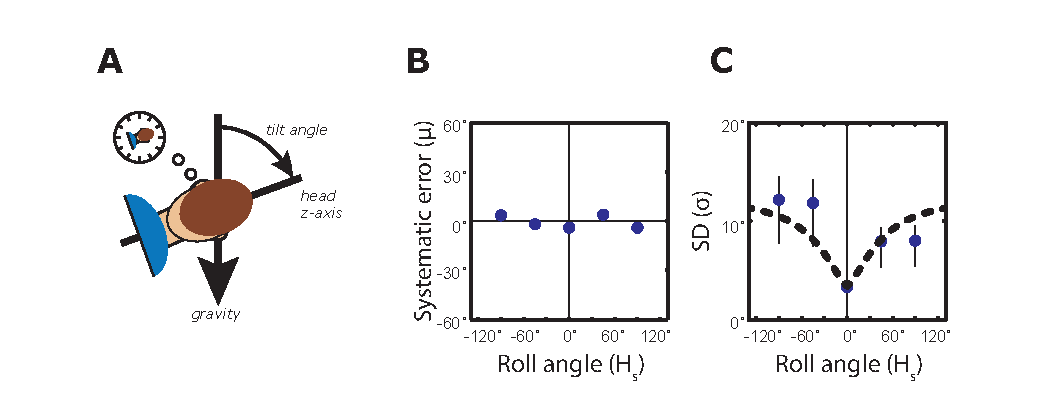
\includegraphics[width=1.0\textwidth]{src/intro/figures/sbt.pdf}

    \caption{Subjective body tilt task (SBT); \panel{A} Graphical representation of the SBT task. \panel{B} Bias and \panel{C} uncertainty as a function of roll angle in a typical participant (circles). The dashed line represents the typical pattern.}
    \label{intro:fig4}
\end{figure}


\subsection{Subjective visual vertical}
The subjective visual vertical, or SVV, task is a similar task in which participants have to judge the orientation of a line with respect to gravity. The PSE, that is the angle at which the line is perceived to be aligned with gravity, can be found by presenting lines at different angles and asking the participant whether the line is rotated clockwise or counter-clockwise relative to gravity (see \panelref{intro:fig5}{A}).

When seated straight this task, participants do not make any static errors and are very certain about their responses (see \panelref{intro:fig5}{B} and \hyperref[intro:fig5]{C}). This changes when tilting the participant before the task. In general, the static error increases with tilt angle. When the direction of the error is in the direction of the body mid-line, this effect is known as the Aubert or A-effect. At smaller angles overcompensation occurs and the static error is in the opposite direction, which is away from the body mid-line. This latter effect is known as the E-effect and could be due to the effects of ocular counter-roll (OCR).

\begin{figure}
    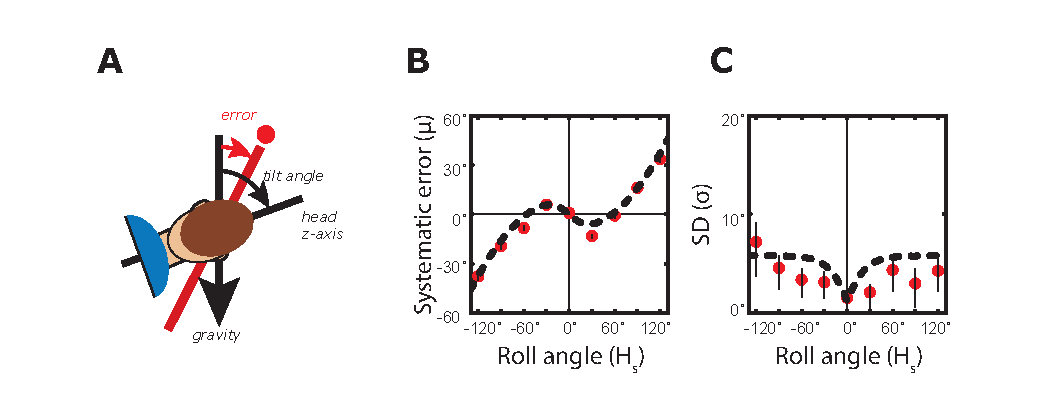
\includegraphics[width=1.0\textwidth]{src/intro/figures/svv.pdf}

    \caption{Subjective visual vertical task (SVV); \panel{A} Graphical representation of the SVV task. \panel{B} Bias and \panel{C} uncertainty as a function of roll angle in a typical participant (circles). The dashed line represents the typical pattern.}
    \label{intro:fig5}
\end{figure}

\subsection{Translation perception}

In the lateral translation task participants had to judge which of two subsequent lateral translations was longest in magnitude. By manipulating one of these translations while keeping the other constant, the effects of these manipulations on self-motion perception can be studied. Because we ask participants to report on the difference between two translations (i.e. longer versus shorter), only relative effects can be assessed.  We used the lateral translation task in \Chapter{p3,p4} to assess the effects of fixation type and distance on self-motion perception.


\section{Outline of this thesis}

Both the estimation of body orientation and self-motion require the integration of multiple sensory signals. This thesis explores how the brain weights and integrates the different sensory signals to form dynamic but coherent percepts of self-motion and orientation.

We start with \Chapter{p1} in which we investigate sensory noise levels of the visual, somatosensory, and vestibular cues to head and body orientation. Because the contributions of these signals cannot be studied in isolation, we adopted an inverse approach where we assumed statistical optimality and attempted to compute the statistical properties of individual sensors. To this end, we fitted an optimal integration model to the behaviour from two psychophyisical tasks. The first gauged head-in-space orientation (SVV) and the second body-in-space orientation (SBT). The resulting estimates of the noise levels in the involved sensory modalities were used to predict the responses of patients with somatosensory and vestibular deficits. These predictions were consistent with previously published deficits in these patient groups, strengthening the idea that human spatial orientation is statistically optimal.

In \Chapter{p3} we examine the dynamic aspects of the integration of vestibular and non-vestibular cues for self-motion perception. We specifically focus on the contributions of eye movements to the perception of whole-body translation. Using a psychophysical task, we first show that translations in which the eyes fixate a body-fixed target are perceived as shorter than those in which the eyes fixate a world-stationary target and thus make pursuit movements. We further demonstrate that this result does not depend on the presence of the fixation point per se, but that the magnitude of unconstrained eye movements in complete darkness directly influences the self-motion percept. 

Because fixation distance influences the magnitude of pursuit eye movements, we investigated  whether the brain takes fixation distance into account in \Chapter{p4}. We compared self-motion perception during gaze fixation on near and far world-fixed targets. Results suggest that fixation depth is only partially taken into account in the integration of vestibular and non-vestibular information for the calculation of translation distance. It seems that only raw eye movements augment self-motion perception, resulting in a biased percept.

An accurate internal estimate of self-motion perception is not only crucial for navigation, but can also be used to updated locations of previously seen objects. This is process in known as spatial updating. \Chapter{p2} presents the final experimental study of this thesis, where we investigate how self-motion signals are used in spatial updating. We show that the errors made during spatial updating do not only depend on the location of the previously seen object, but also on the location of gaze. This is consistent with spatial updating in a gaze-centred reference frame. We further show that the underestimation of self-motion is a possible cause of the errors found.
